\section{SVM}
Support vector machines is a supervised learning method that analyzes the data 
and tries to recognize patterns, within the classification domain.
 The standard SVM method is an binary classifier, which predicts for a given 
input which class the input belongs two. 
 Prediction is done based on the model it builds from the training session, the 
model provides a "clear gap" that provide the distinction between the first or 
the latter class. \\

Support vector machine constructs a hyperplane or set of hyperplanes in a high 
dimension. 
The hyperplane that has the largest distance to the nearest training data points 
of any class (so-called functional margin), provides the best separation,  since 
it result it a clear distinction between the classes, and lower general error.
\\

The goal in SVM is to find this hyperplane which provides the optimal separation 
of the classes by having the widest margin. 

\begin{figure}[H]
\centering
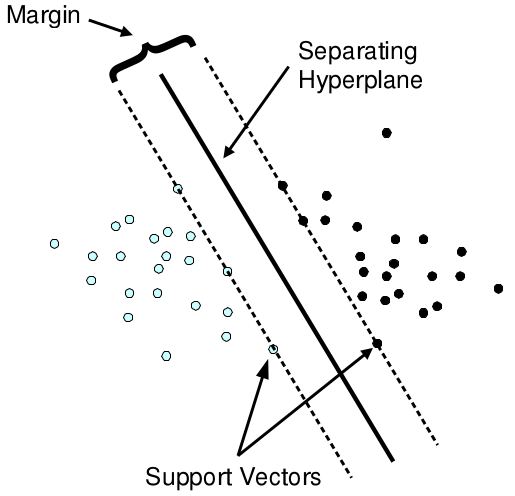
\includegraphics[width = 0.5\textwidth]{img/SVM-illu.png}
\caption{Svm Illustrated}
\label{fig::SVM-illustrated}
\end{figure}

The training data for this method consist a set of input vectors denoted as 
$\mathbf{x_i}$, each input vector has a number of component features. Each input 
vector is given a label, indicating its class.

The hyperplane is given as 
\begin{equation}
\mathbf{w} \cdot \mathbf{x} + b = 0
\end{equation}

In which the $\mathbf{w}$ determines the orientation of the plane, and 
$\mathbf{b}$ is the offset of the plane from the origin. \\
 
The seperaing hyperplane which maximizes the margin can be found by examining 
the convex hull of each class’s training data  and then find the closest points 
in the two convex hulls. The convex hull of a set of points is the
smallest convex set containing the points.  If the hyperplane that bisects both 
convex hulls can be found, will the resulting classifier deemed robust in some 
sense. 

\begin{figure}[H]
\centering
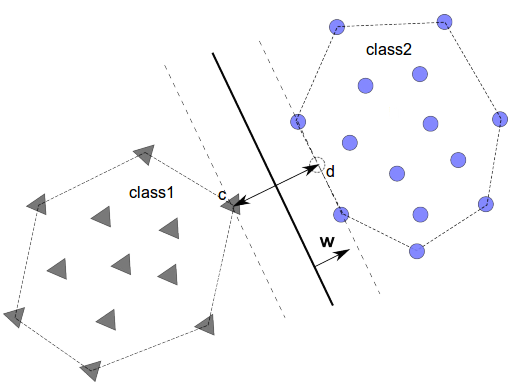
\includegraphics[width = 0.5\textwidth]{img/convex_hull.png}
\caption{Best plane bisects closest points in the convex hulls,The convex hulls 
are labeled c and d}
\label{fig::convex_hull}
\end{figure}  

To find  the plane, one have to find the points closest to the plane, which can 
be found by solving the quadratic problem. \\ 

\begin{equation}
min_\alpha~\left(\frac{1}{2} ||c-d||^2\right)
\end{equation}

where c and d are the closest to be found points, these are defined as 
\begin{equation}
\begin{aligned}
&c = \sum_{y_i~\in~class1} \alpha_ix_i  
& \text{subject to}
&& \sum_{y_i~\in~class1}\alpha_i =1 
&& \alpha_i \geq 0
\end{aligned} 
\end{equation}

\begin{equation}
\begin{aligned}
&d = \sum_{y_i~\in~class2} \alpha_ix_i  
& \text{subject to}
&& \sum_{y_i~\in~class2}\alpha_i =1 
&& \alpha_i \geq 0
\end{aligned} 
\end{equation}


An alternative approach involves a search through the space of every possible 
hyperplane in order to find a set of two parallel planes that divide the points 
into homogeneous groups yet themselves are as far apart as possible.\\


In the case of non-linearly separable data, can a linear hyperplane not be used 
to define the solution. 
For this purpose is a slack variable introduced, which allows some points on the 
incorrect side of the margin, creating a soft margin, when a linear hyperplane 
was used to separate them.\\

A different approach for solving this problem would be using the kernel trick. 
The kernel trick involves transforming in $\mathbb{R}^n \rightarrow 
\mathbb{R}^{n+1}$. 
The challenging part is to find such transformation, $\phi$ which allow 
transforming data into a higher dimension. 

Kernel functions are in general in the following form:
\begin{equation}
K(\overrightarrow{x_i},\overrightarrow{x_j}) = \phi(\overrightarrow{x_i}) \cdot 
\phi(\overrightarrow{x_j}) 
\end{equation}

$x_i$ and $x_j$ illustrates two different feature vectors. 

Different kernels does already exist, and may already be implemented in 
different SVM software packages. 
\\

\textbf{Linear kernel}:
\begin{equation}
K(\overrightarrow{x_i},\overrightarrow{x_j}) = (\overrightarrow{x_i}) \cdot 
(\overrightarrow{x_j}) 
\end{equation}

Linear kernel does not transform the data, but computes the dot product. 
\\

\textbf{Polynomial kernel of degree $d$}:
\begin{equation}
K(\overrightarrow{x_i},\overrightarrow{x_j}) = ((\overrightarrow{x_i}) \cdot 
(\overrightarrow{x_j})+1)^d
\end{equation}

The Polynomial kernel adds a nonlinear transformation of the data.
\\

\textbf{Sigmoid kernel}
\begin{equation}
K(\overrightarrow{x_i},\overrightarrow{x_j}) = tanh( k(\overrightarrow{x_i}) 
\cdot (\overrightarrow{x_j}) - \delta)
\end{equation}
\\

\textbf{Radial basis function kernel}
\begin{equation}
K(\overrightarrow{x_i},\overrightarrow{x_j}) =  
exp\left(\frac{||\overrightarrow{x_i} - 
\overrightarrow{x_j}||}{2\sigma^2}\right)
\end{equation}

In which the value $\gamma = \frac{1}{2\sigma^2}$ can be adjusted.\\


The choice of kernel depends what kind of transformation is needed. 
